\subsection{Layered protocols}
The \textit{layered protocols} are protocols in which there is a clear division between different layers. Every layer has a specific function and we can say that each layer speaks with the corresponding layer on the other side.

\subsubsection{OSI model}
An example of \textit{layered protocol} is the \textit{OSI model}. As we can see from \textit{Figure 1}, we have several levels, each of which plays a specific role. 

\begin{figure}[h]
\caption{OSI model}
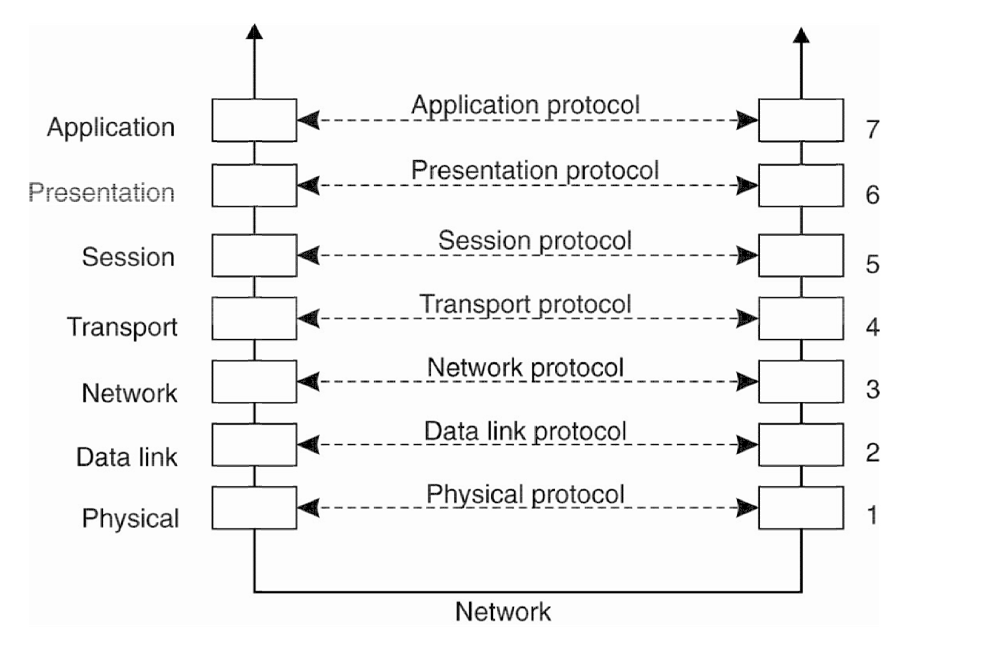
\includegraphics[width=\textwidth]{src/images/osi-model.png}
\centering
\end{figure}

In the \textit{OSI model} we distinguish between three different kinds of layers.
\begin{itemize}
    \item \textbf{Low layers}
        \begin{itemize}
            \item \textit{Physical layer}: it describes the bit transmission
            \item \textit{Data link layer}: it describes the organization of the series of bits into frames
            \item \textit{Network layer}: it describes how packets have to be routed
        \end{itemize}
    \item \textbf{Transport layer}
        \begin{itemize}
            \item It describes how data is transmitted
            \item \unserline{It offers a service independent from the lower layers}
            \item It provides the actual communication facilities for most distributed systems
        \end{itemize}
        The main standards are \textbf{TCP} \textit{(connection-oriented, reliable, stream-oriented communication)} and \textbf{UDP} \textit{(unreliable datagram communication)}
    \item \textbf{Higher level layers}\\
        They are \textit{session, presentation and application} layers and typically they are merged together.
\end{itemize}
Another important concept is the \textit{encapsulation}. As the image above can suggest, every layer is encapsulated by the lower one.

\subsubsection{Middleware as a protocol layer}
We can consider \textit{middleware} as a protocol layer in the sense that they include common services and protocols that can be used by different applications. In practice, it can:
\begin{itemize}
    \item Implement \textit{marshaling} and \textit{unmarshaling} data procedures
    \item Implement naming protocols in order to allow sharing of resources
    \item Implement security protocol for secure communication
    \item Implement scaling mechanism, such as for replication and caching
\end{itemize}

\subsection{Remote procedure call}
In a \textbf{local procedure call} the parameters are passed through stack. The caller writes the parameters in the stack and then call the procedure. The called simply read the parameters from the stack since the memory is shared.\\
There are different ways to pass parameters to a procedure:
\begin{itemize}
    \item \textit{By value}: C-like when passing basic data types
    \item \textit{By reference}: Java-like when passing objects
    \item \textit{By copy/restore}: it's similar but slightly different than previous one. Value is passed in and has no effect on the value of the variable passed in until the end of the function, at which point the final value of the function variable is stored in the passed in variable.\\
    The basic difference between \textit{call by reference} and \textit{copy/restore} then is that changes made to the function variable will not show up in the passed in variable until after the end of the function while call by reference changes will be seen immediately.
\end{itemize}

\begin{figure}[h]
\caption{RPC in detail}
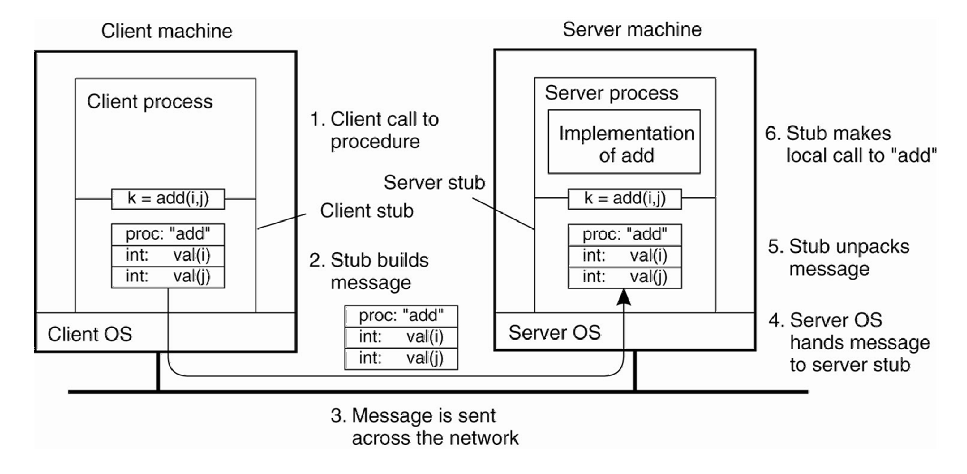
\includegraphics[width=\textwidth]{src/images/rpc-in-detail.png}
\centering
\end{figure}

\subsubsection{Marshalling and serialization}

Two problems when passing parameters:
\begin{itemize}
    \item Structured data must be ultimately flattened in a byte stream: \textbf{serialization}
    \item Hosts may use different data representations \textit{(e.g., little endian vs. big endian, EBCDIC vs. ASCII)} and proper conversions are needed: \textbf{marshalling}
\end{itemize}
In order to simplify the procedure, these operations are done by the middleware, helped by:

\begin{itemize}
    \item \textbf{IDL} \textit{(Interface Definition Language)}: a language and platform independent representation of the procedure's signature
    \begin{itemize}
        \item It raises the abstraction level of the service definition
        \item The language comes with "mappings" onto target languages
        \item It can also be used to automatically generate the service interface code in the target language 
    \end{itemize}
    \item A data representation format to be used during communication
\end{itemize}

\subsubsection{Sun Microsystems' RPC}
\begin{itemize}
    \item Also called \textit{Open Network Computing RPC}
    \item Data format is specified by \textit{XDR (eXternal Data Representation)}
    \item \textbf{Parameters are passed by value}
    \item It can use TCP or UDP
    \item Security is provided through \textit{DES}
\end{itemize}

\subsubsection{Distributed Computed Environment (DCE)}
\begin{itemize}
    \item It's a set of specifications and a reference implementation
    \item Several invocation semantics are offered
    \item Several services are provided on top of RPC
    \begin{itemize}
        \item Directory service
        \item Distributed time service
        \item Distributed file service
    \end{itemize}
    \item Security is provided through \textit{Kerberos}
\end{itemize}

\subsubsection{Binding client to server}
One of the main problems is find out which server provides a given service and how to establish communication with it and, obviously, it's undesirable to hard-writing this info in the client code.

\textbf{Sun's solution}
\begin{itemize}
    \item Introduce a daemon called \textit{portmap} that binds calls and server/ports
    \item It's important to notice that \textit{portmap} provides its services only to local clients, i.e., it solves only the problem of establish the communication
    \begin{itemize}
        \item In fact, the client must know in advance where the service resides
    \end{itemize}
    \item In order to bypass this limitation, the client can send multicast message to many \textit{portmap} daemons
\end{itemize}

\textbf{DCE's solution}
\begin{itemize}
    \item The DCE daemon works like \textit{portmap}
    \item Client doesn't need to know in advance where the service is: the only need to know where the directory service is
    \begin{itemize}
        \item The directory service can be distributed
    \end{itemize}
    \item Then, the daemon solves both the problem to find a service and establish a communication with it
\end{itemize}

\paragraph{Dynamic activation}
he server processes may remain active even in absence of requests, wasting resources. A possible solution to this problem is to introduce another (local) server daemon that:
\begin{itemize}
    \item Forks the process to serve the request
    \item Redirects the request if the process is already active
\end{itemize}
With this system, however, we have a disadvantage: the first request is served less efficiently.

\subsubsection{Lightweight RPC}
Using a conventional \textit{RPC}, sometimes, is not the better solution. For example, if we have a TCP/UDP service on the same machine a conventional \textit{RPC} would lead to wasted resources.\\
For this reason it's born the a kind of simplified \textit{RPC}, called \textit{lightweight RPC}.\\
The idea is to pass messages through local facilities, i.e. communication exploits a private shared memory region.\\
The \textit{invocation} procedure is the following:
\begin{enumerate}
    \item Client copies parameters in the shared stack and performs the system call
    \item Kernel does a context switch, to execute the procedure in the server
    \item Results are copied on the stack and another system call
    \item Context switch brings execution back to the client
\end{enumerate}
With this procedure the main advantage is that we use less threads/processes (no need to listen on a channel).

\subsubsection{Async RPC}
In a parallel system (or, more in general, in a non-distributed system), when a call is performed, the caller is suspended until the callee is done. \textit{RPC} preserves this behaviour but it can, potentially, wastes client resources.
For this reason we introduce the \textit{Async RPC}, in which the caller is not suspended and it can continue in other operations.\\
There are many variant of \textit{async RPC}:
\begin{itemize}
    \item If no result is needed execution can resume after an \textit{ack message} is received from the server
    \begin{figure}[h]
        \caption{Asynchronous}
        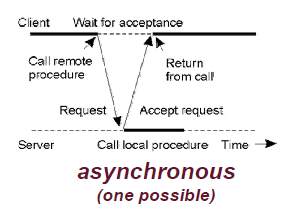
\includegraphics[scale=0.6]{src/images/async.png}
        \centering
    \end{figure}

    \item The callee may (async) invoke the caller back or invocation may return immediately a \textit{promise}
    \begin{figure}[h]
        \caption{Deferred synchronous}
        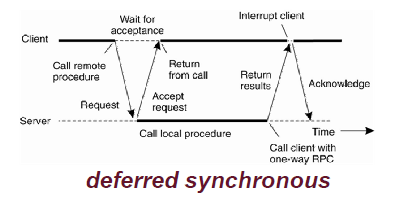
\includegraphics[scale=0.6]{src/images/deferred-synchronous.png}
        \centering
    \end{figure}
\end{itemize}

\subsubsection{Batched vs. queued RPC}
\textit{Sun RPC} includes the ability to perform \textit{batched RPC}. RPCs that do not require a result are buffered on the client and they are sent all together when a non-batched call is required or when a timeout expires. It's important to notice that this mechanism enables yet another form of \textit{async RPC}.
